\begin{solution}{normal}
Heat leaving the room in stable state is equal to heat produced by heater by Fourier's law.
$$P(T_2) = k(T_2-T_1)$$
In the second case,
$$ P(T_4) = k(T_4-T_3)$$
Therefore, point $(T_4,P(T_4))$ must be on the line which passes through point $(T_3,0)$ with the same slope as the line passing through $(T_2,P(T_2))$ and $(T_1,0)$
This gives $\boxed {T_4=1.4T_3}$
\begin{center}
    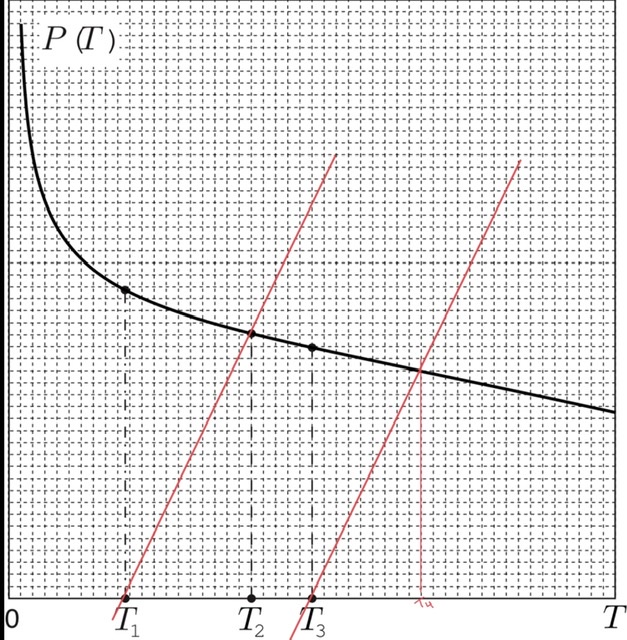
\includegraphics[width=8cm]{t38.jpeg}
\end{center}
\end{solution}